% Slides accompanying "Learn RISC-V CPU Implementation and BSV" book
% Copyright (c) 2024 Rishiyur S. Nikhil, All Rights Reserved

% -*- mode: fundamental -*-

% Slides accompanying "Learn RISC-V CPU Implementation and BSV" book
% Copyright (c) 2024 Rishiyur S. Nikhil, All Rights Reserved

% This is a preamble shared by all the slide decks

\documentclass[10pt, aspectratio=169]{beamer}

% \documentclass[17pt]{beamer}

% Avail. font sizes: 8pt, 9pt, 10pt, 11pt, 12pt, 14pt, 17pt, 20pt.
% Default font size is 11pt (= 22pt in full screen mode).

\usepackage{verbatim}
\usepackage{fancyvrb}
\usepackage{listings}

% ================================================================
% Themes

\usetheme{Madrid}          % Line at bottom: Author (affiliation), OptTitle, Conf, page 

% \usetheme{Copenhagen}    % Same as Madrid except bottom line: Author, OptTitle

% \usetheme{Berkeley}    % Takes up 1-inch border on left and top

% ----------------
% colorthemes
% (default), beaver, beetle, seahorse, wolverine

\usecolortheme{seahorse}

% ================================================================
% Customization: show table of contents before each section
% Use \AtBeginSubsection    to show before each subsection

% \AtBeginSection[]
% {
%   \begin{frame}
%     \frametitle{Table of Contents}
%     \tableofcontents[currentsection]
%   \end{frame}
% }

% ================================================================

% ----------------
% The bsc compiler and BSV language
\newcommand{\bsc}{\emph{bsc}}
\newcommand{\BSV}{\bf{BSV}}
% ----------------
% ITALICISE WORDS
\newcommand{\ie}{\emph{i.e.,}}
\newcommand{\eg}{\emph{e.g.,}}
\newcommand{\Eg}{\emph{E.g.,}}
\newcommand{\etc}{\emph{etc.}}
\newcommand{\via}{\emph{via}}
\newcommand{\vs}{\emph{vs.}}

% ----------------
% EMPTY BOXES OF VARIOUS WIDTHS, FOR INDENTATION

\newcommand{\hm}{\hspace*{1em}}
\newcommand{\hmm}{\hspace*{2em}}
\newcommand{\hmmm}{\hspace*{3em}}
\newcommand{\hmmmm}{\hspace*{4em}}

% ----------------
% Convenient widths

\newlength{\hlessmm}
\setlength{\hlessmm}{\textwidth}
\addtolength{\hlessmm}{-2em}

\newlength{\hlessmmm}
\setlength{\hlessmmm}{\textwidth}
\addtolength{\hlessmmm}{-3em}

\newlength{\hlessmmmm}
\setlength{\hlessmmmm}{\textwidth}
\addtolength{\hlessmmmm}{-4em}

% ================================================================
% Title page

\title[Learn CPU design \& BSV]{Learn RISC-V CPU Implementation and BSV}

\subtitle{(BSV: a High-Level Hardware Design Language)}

\author[{\copyright} R.S.Nikhil]{Rishiyur S.~Nikhil}
% \institute{Bluespec, Inc.}

% Date is set differently in each slide deck

% \logo{
\includegraphics[height=0.6cm]{../Figures/Bluespec_Logo_2022-10}}

% End of preamble
% ****************************************************************


\date{L17: {\BSV}: Tighter Rule scheduling with CRegs}

% ****************************************************************

\begin{document}

% ================================================================

\begin{frame}
\titlepage

\begin{center}
 
\includegraphics[height=1cm]{Bluespec_Logo_2022-10}
\end{center}

\end{frame}

% ================================================================

\section{Reminders}

% -*- mode: fundamental -*-

% ================================================================

\begin{frame}[fragile]
\frametitle{Reminders}

\footnotesize

Please git clone: \url{https://github.com/rsnikhil/Learn_Bluespec_and_RISCV_Design} \\
(git pull for latest version).  Repsitory structure:

\vspace{1ex}

\begin{minipage}{0.5\textwidth}\scriptsize
\begin{Verbatim}[frame=single, numbers=left]
    ./Book_BLang_RISCV.pdf
      Slides/
          Slides_01_Intro.pdf
          Slides_02_ISA.pdf
          ...
      Exercises/
          Ex-03-A-Hello-World/
          Ex-03-B-Top-and-DUT/
          ...
      Code/
          src_Top/
          src_Drum/
          src_Fife/
          src_Common/
          ...
      Doc/Installing_bsc_Verilator_etc.{adoc,html}
\end{Verbatim}
\end{minipage}
\hm
\begin{minipage}{0.45\textwidth}
\begin{itemize}

 \item Slides and Exercise are numbered in sync with book Chapter numbers.

 \item For Exercises, please see Appendix E of the book.  Some (not
       all) exercises have associated code in the {\tt Exercises/}
       directory.

\end{itemize}
\end{minipage}

\vspace{2ex}

To compile and run the code for exercises, Drum and Fife, please make sure you have installed:

\begin{itemize}

 \item \emph{bsc} compiler (see \url{https://github.com/B-Lang-org/bsc})

 \item Verilator compiler (see \url{https://www.verilator.org/})
\end{itemize}

\footnotesize

\end{frame}

% ================================================================

\begin{frame}
\frametitle{Chapter Roadmap}

\footnotesize

\begin{center}
\frame{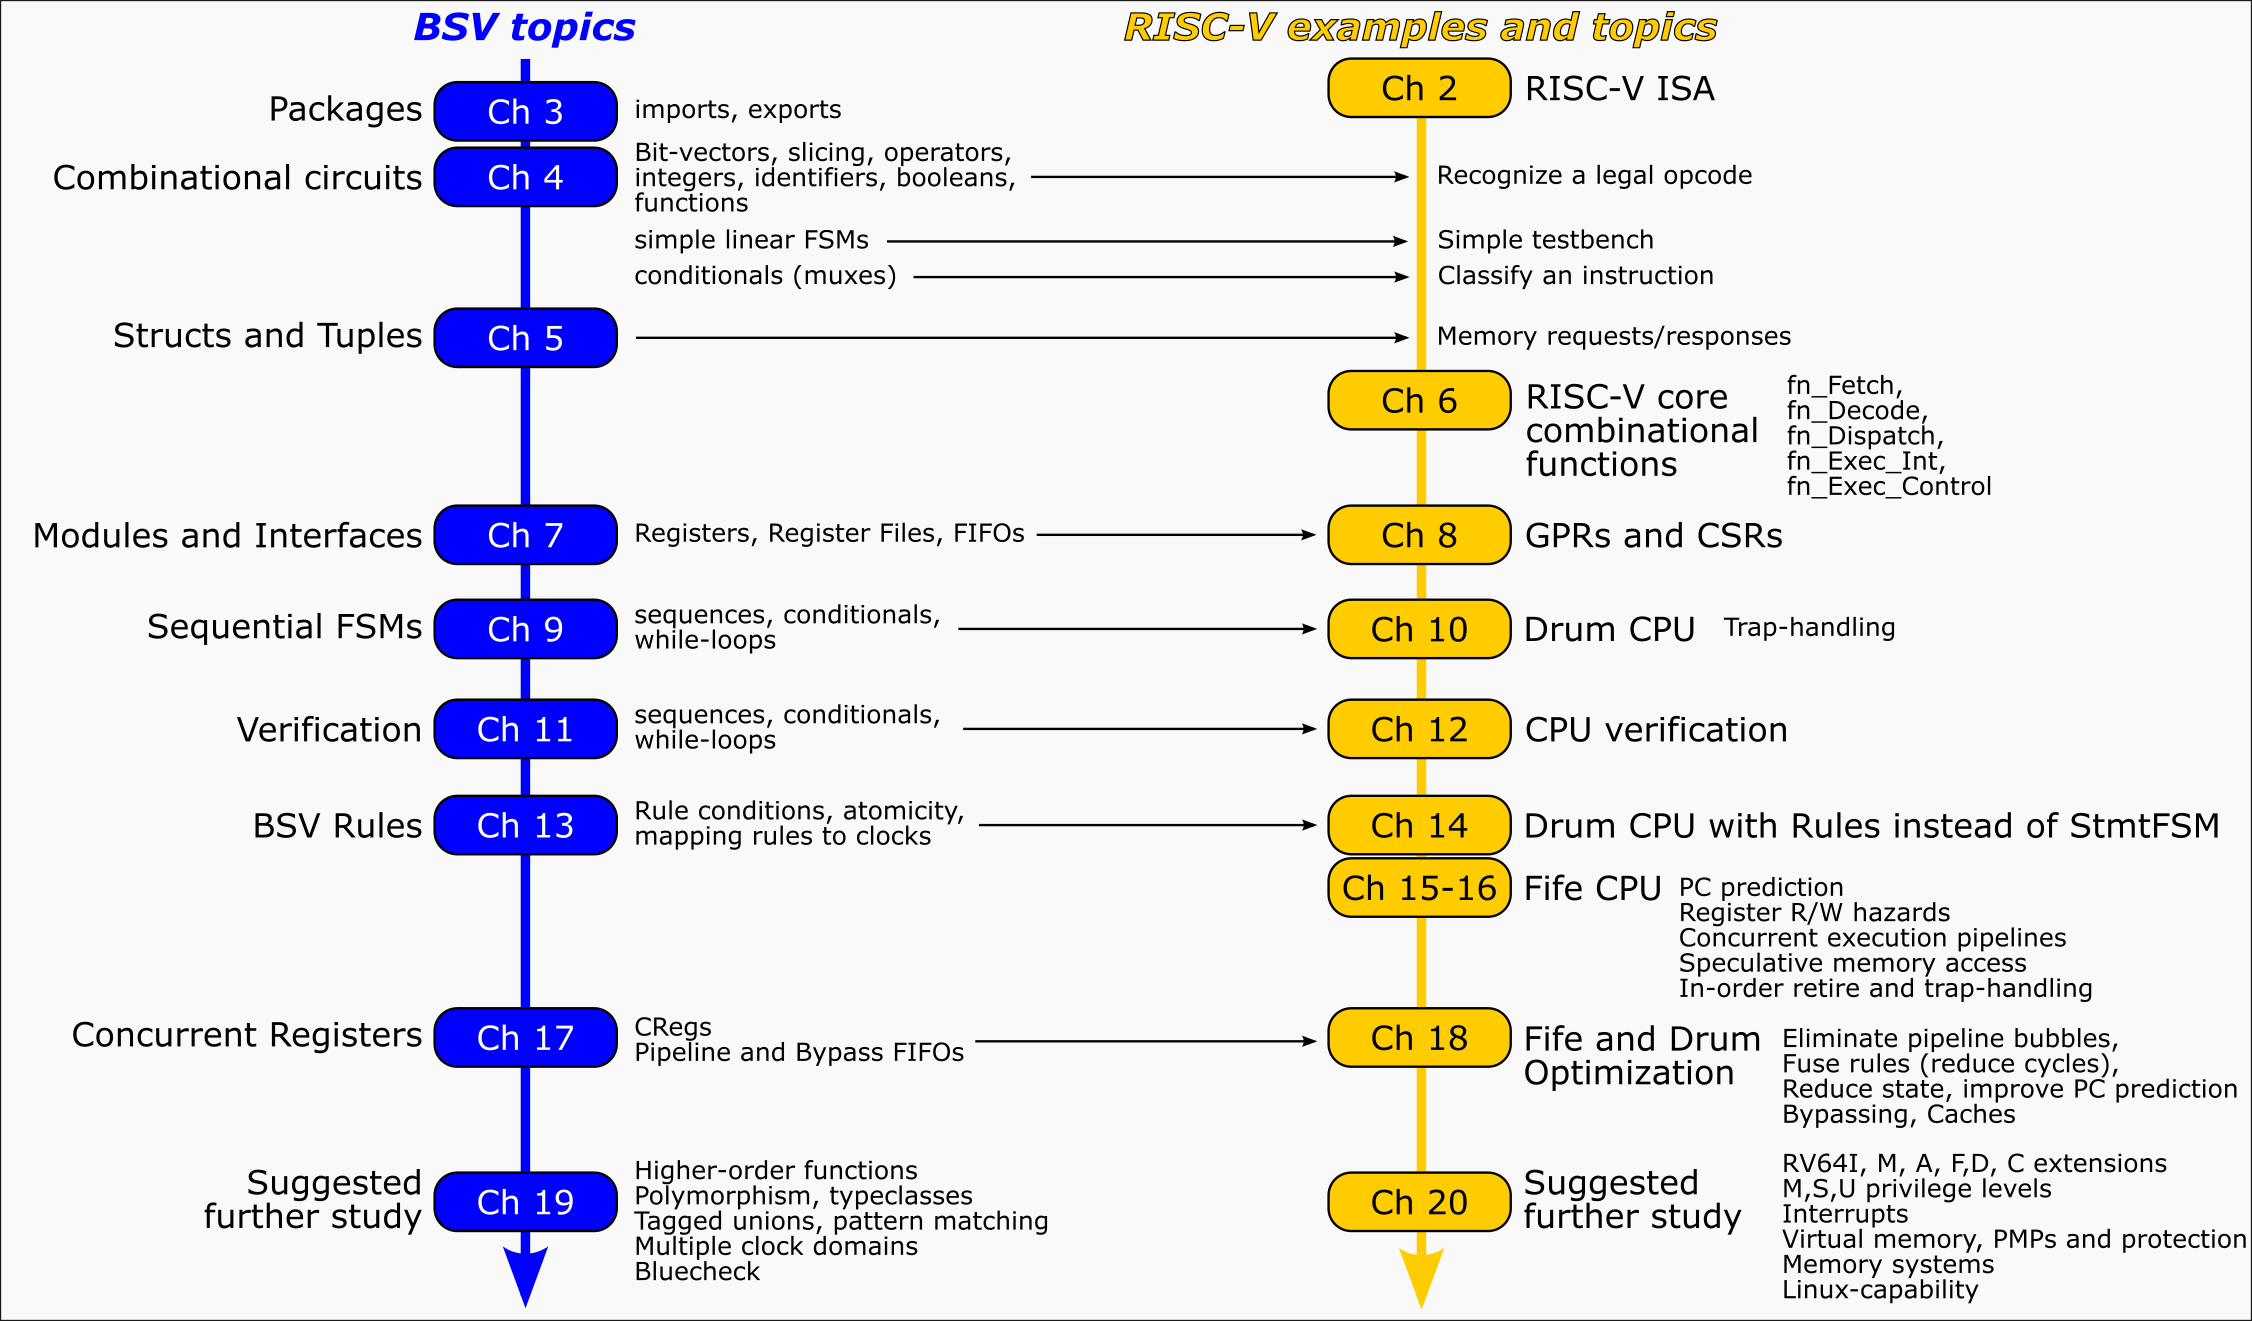
\includegraphics[height=0.825\textheight]{Fig_Chapter_Roadmap}}
\end{center}

\end{frame}

% ================================================================


% ================================================================

\begin{frame}
\frametitle{Table of Contents}

\tableofcontents

\end{frame}

% ****************************************************************

\section{Motivation}

\begin{frame}

\begin{center}
  {\LARGE BSV: Tighter Rule Scheduling: Motivation}
\end{center}

\end{frame}

% ================================================================

\begin{frame}[fragile]
\frametitle{Tighter Rule Scheduling: Motivation}

\footnotesize

\begin{tabular}{ | c | p{0.55\textwidth} | p{0.35\textwidth} | }
 \hline
   \hm & {\BSV} & \scriptsize \emph{Analogy: RISC-V ISA} \\
 \hline
 \hline
     (A)

   & Rule semantics are abstract: one rule at a time

   & \scriptsize \emph{RISC-V ISA semantics are abstract: one instruction at a time}

   \\

 \hline
     (B)

   & When the {\bsc} compiler maps a set of rules to execute
     simultaneously (in the same clock), all their methods occur at
     the same instant (clock edge). All ``read-values'' are from the
     previous clock edge; all ``write-values'' ({\tt Action} and {\tt
     ActionValue} results) are visible only at the next clock edge.

     \vspace{1ex}

     {\bsc} must ensure that the \emph{ordering} of methods in (B) is
     consistent with (A).

     \vspace{1ex}

     In particular, {\bsc} may introduce (combinational) control
     circuits to \emph{stall} a rule to avoid violating (A).

   & \scriptsize

     \emph{RISC-V instructions can be executed in pipelines, in parallel
     (superscalar), out-of-order, ...  The implementation must ensure
     that the \emph{order} in which they retire, and the \emph{order} in
     which they read and write registers and memory, is consistent
     with (A).

     \vspace{1ex}

     In particular, an instruction may be \emph{stalled} to avoid
     violating (A).}

   \\
 \hline
\end{tabular}

\end{frame}

% ================================================================

\subsection{Motivational Example}

\begin{frame}[fragile]
\frametitle{Tighter Rule Scheduling: Motivational Example: Up-Down Counter (1/2)}

\footnotesize

This is an interface for an ``Up-Down'' Counter:

\begin{Verbatim}[frame=single]
interface Up_Down_Counter_IFC;
   method Action   init (Bit #(4) init_val);
   method Bit #(4) val;
   method Action   decr;
   method Action   incr;
endinterface
\end{Verbatim}

\vspace{2ex}

Example usage: ``Credit-based'' flow control in a network interface (NI):
\begin{itemize}

 \item NI sends stream of packets to remote receiver, which can buffer up to $N$ packets.
 \item Remote receiver sends stream of packet-acknowledgements back to NI.
 \item These two streams are asynchronous and concurrent.

 \vspace{4ex}

 \item Initialize counter to $N$ (available space in remote buffer)
 \item Send packet only if counter value $> 0$ (stall otherwise)
 \item Decrement counter for each packet sent
 \item Increment counter for each packet-acknowledgment received

\end{itemize}

\end{frame}

% ----------------------------------------------------------------

\begin{frame}[fragile]
\frametitle{Tighter Rule Scheduling: Motivational Example: Up-Down Counter (2/2)}

\footnotesize

Here is a possible implementation of an ``Up-Down'' Counter:

\begin{minipage}{0.55\textwidth}\scriptsize
\begin{Verbatim}[frame=single]
module mkUp_Down_Counter_I (Up_Down_Counter_IFC);
   // STATE
   Reg #(Bit #(4)) rg_counter <- mkReg (15);

   // --------------------------------
   // INTERFACE

   method Action init (Bit #(4) init_val);
      rg_counter <= init_val;
   endmethod

   method Bit #(4) val;
      return rg_counter;
   endmethod

   method Action decr () if (rg_counter != 0);
      rg_counter <= rg_counter - 1;
   endmethod

   method Action incr () if (rg_counter != 15);
      rg_counter <= rg_counter + 1;
   endmethod
endmodule
\end{Verbatim}
\end{minipage}
\hm
\begin{minipage}{0.4\textwidth}

Analysis: Rules invoking {\tt .incr()} and {\tt .decr()} cannot execute on the same clock edge.

\begin{itemize}\scriptsize

 \item (A) In the abstract rule semantics, either {\tt .incr()}
       precedes {\tt .decr()} or \emph{vice versa}.

       \vspace{1ex}

       In either case, the latter rule observes the update from the previous rule.

       \vspace{4ex}

 \item (B) If they executed on the same clock, neither rule sees the
       update from the other rule.  This is inconsistent with (A).

\end{itemize}

\vspace{1ex}

{\scriptsize
Consequently, this implementation cannot send a packet (decr) and
register an ack (incr) in the same clock, even though the two streams
are asynchronous and concurrent.}

\vspace{1ex}

{\scriptsize
On the average, we can only send (and register ack) on every alternate clock.}

\vspace{2ex}

{\bf Solution:} \\
Use a \emph{Concurrent Register} ({\tt CReg}) for {\tt rg\_counter}.

\end{minipage}

\end{frame}

% ****************************************************************

\section{Concurrent Registers}

\begin{frame}

\begin{center}
  {\LARGE BSV: Concurrent Registers ({\tt CReg}s)}
\end{center}

\end{frame}

% ================================================================

\subsection{CRegs}

\begin{frame}[fragile]
\frametitle{CRegs}

\footnotesize

A Concurrent Register, or \verb|CReg|, is a module provided by
 the \emph{bsc} library.  Its interface is an \emph{array}
 of \verb|Reg#(t)| interfaces:

\begin{Verbatim}[frame=single]
module mkCReg #(parameter Integer n,
                parameter a_type resetval)
              (Reg#(a_type) ifc[])
\end{Verbatim}

\vspace{5ex}

It is instantiated similar to this example: \\
(This example: register content type: \verb|Bit#(4)|; initial value: 15; 2 {\tt Reg} interfaces).

\begin{Verbatim}[frame=single]
   // parameter n is 2, resetval is 15
   Array #(Reg #(Bit #(4))) crg_counter <- mkCReg (2, 15);
\end{Verbatim}

\end{frame}

% ================================================================

\subsection{Hardware intuition}

\begin{frame}[fragile]
\frametitle{Hardware intuition for a CReg}

\label{slide_hw_intuition}

\footnotesize

\begin{center}
 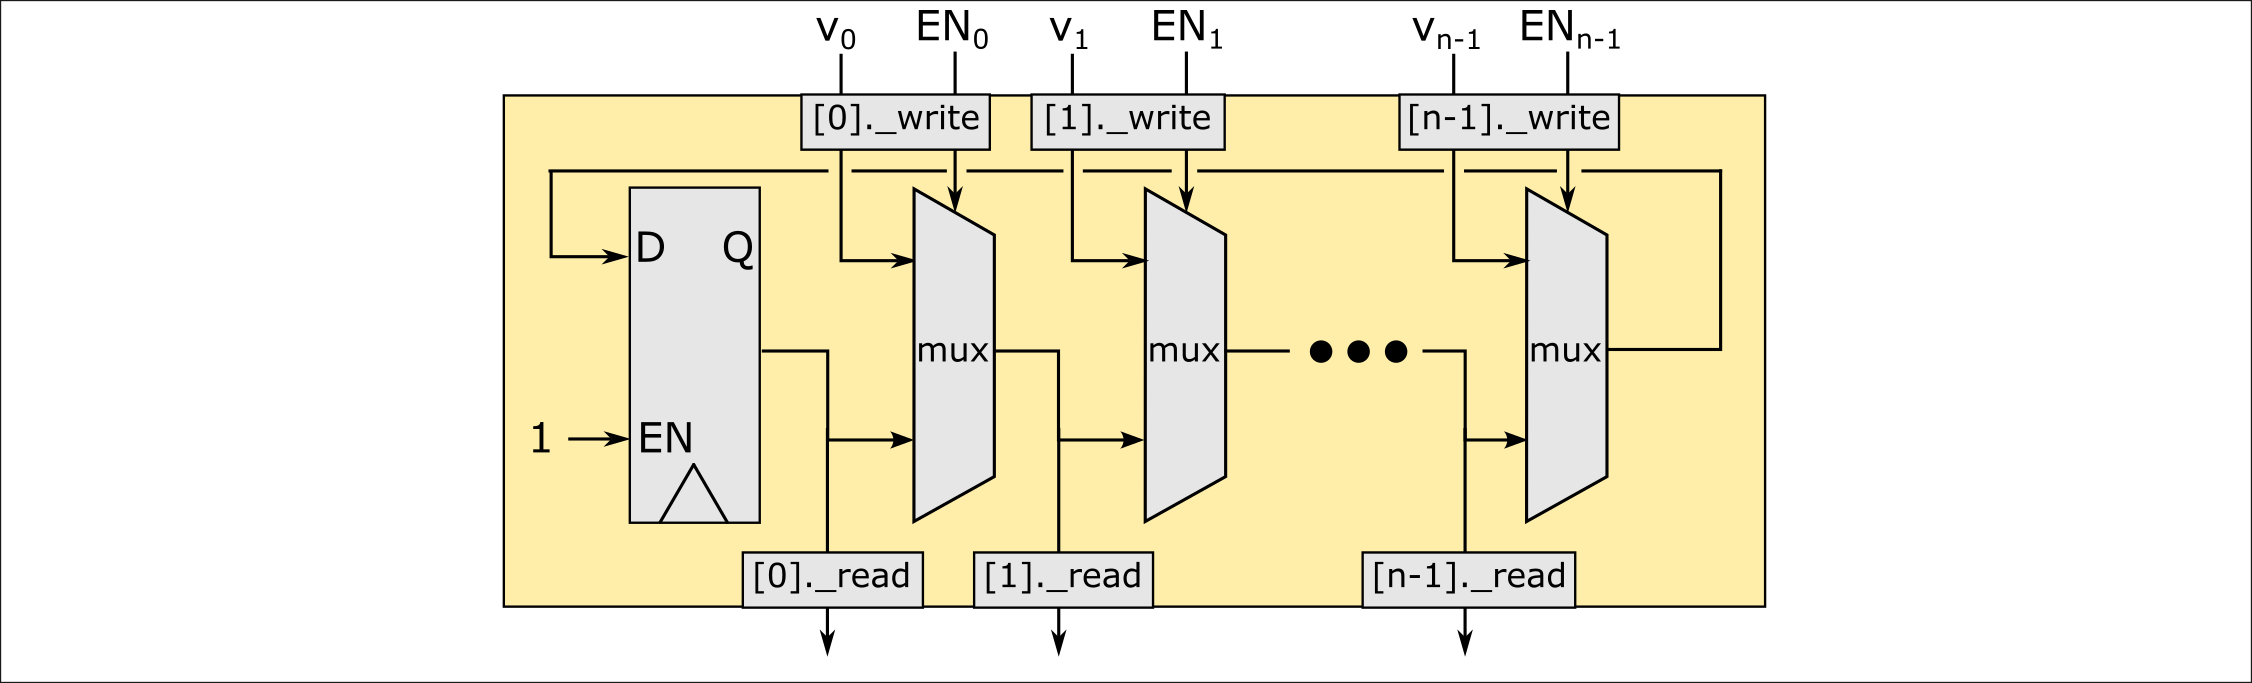
\includegraphics[width=\textwidth]{Fig_CReg_HW}

 \vspace{1ex}

 This has an array of $n$ {\tt Reg} interfaces, indexed from 0 to $n$-1.

 \vspace{1ex}

 The $j$'th interface has {\tt [$j$].\_read()} and {\tt [$j$].\_write()} methods.
\end{center}

\end{frame}

% ================================================================

\subsection{CReg ordering properties}

\begin{frame}[fragile]
\frametitle{CReg ordering properties}

\footnotesize

\fbox{
\begin{minipage}{0.6\textwidth}
\begin{itemize}

 \item All the methods can be invoked in the same clock.

 \item A read at the $j$'th register interface,{\ie} {\tt x[$j$].\_read}
       returns the latest of:

       \begin{itemize}\footnotesize
        \item the value in the register;
        \item if {\tt x[0].\_write($v_0$)} is being invoked, the value $v_0$;
        \item if {\tt x[1].\_write($v_1$)} is being invoked, the value $v_1$;
        \item ...
        \item if {\tt x[$j-1$].\_write($v_{n-1}$)} is being invoked, the value $v_{n-1}$;
       \end{itemize}

 \item The register value is updated with the latest of:

       \begin{itemize}\footnotesize
        \item the current value in the register;
        \item if {\tt x[0].\_write($v_0$)} is being invoked, the value $v_0$;
        \item if {\tt x[1].\_write($v_1$)} is being invoked, the value $v_1$;
        \item ...
        \item if {\tt x[$n-1$].\_write($v_{n-1}$)} is being invoked, the value $v_{n-1}$;
       \end{itemize}

\end{itemize}
\end{minipage}}
\hm
\begin{minipage}{0.35\textwidth}

This ordering corresponds exactly to the left-to-right and
top-to-bottom ordering of the methods in the hardware-intuition
diagram (Slide~\ref{slide_hw_intuition}).

\end{minipage}

\end{frame}

% ================================================================

\subsection{Up-down counter with CReg}

\begin{frame}[fragile]
\frametitle{Up-down counter with a CReg}

\footnotesize

\begin{minipage}{0.5\textwidth}\scriptsize
\begin{Verbatim}[frame=single]
module mkUp_Down_Counter_I (Up_Down_Counter_IFC);
   // STATE
   Array #(Reg #(Bit #(4))) crg_counter <- mkCReg (3,15);

   // --------------------------------
   // INTERFACE
   method Action init (Bit #(4) init_val);
      crg_counter [2] <= init_val
   endmethod

   method Bit #(4) val;
      return rg_counter [0];
   endmethod

   method Action decr if (rg_counter != 0);
      rg_counter [1] <= rg_counter [1] - 1;
   endmethod

   method Action incr if (rg_counter != 15);
      rg_counter [0] <= rg_counter [0] + 1;
   endmethod
endmodule
\end{Verbatim}
\end{minipage}
\hm
\begin{minipage}{0.45\textwidth}
 Some questions to ponder:

 \begin{itemize}

  \item What does method {\tt val} return? \\
        \hm The original value in the register? \\
        \hm The value after the increment? \\
        \hm The value after the decrement? \\
        \hm The value after the increment and decrement?

  \item What happens if methods {\tt incr} and {\tt decr} are called
        simultaneously?  Which one happens (semantically) ``first''?

        Note: {\tt incr} saturates at 15, and {\tt decr} saturates at
        0, so the order matters!

 \end{itemize}

 \vspace{2ex}

 \emph{Hint:} The answers are in the choice of {\tt CReg} indexes in each method.
\end{minipage}

\end{frame}

% ================================================================

\subsection{Example: CSR {\tt mcycle} in RISC-V}

\begin{frame}[fragile]
\frametitle{Example: CSR {\tt mcycle} in RISC-V}

\footnotesize

CSR {\tt mcycle} (RISC-V CPU cycle counter) is updated by two ``processes'':

\begin{itemize}

 \item (A) Standalone infinite loop incrementing {\tt mcycle} on every cycle.

 \item (B) Instruction execution, when we have a {\tt CSRRxx} instruction
           that writes to {\tt mcycle}.
\end{itemize}

The RISC-V spec says that when (B) happens, it should override (A).

\PAUSE{\vspace{5ex}}

We can instantiate a CReg for this:

\vspace{1ex}

\begin{Verbatim}[frame=single, label=from src\_Common/CSRs.bsv]
   Array #(Reg #(Bit #(64))) csr_mcycle <- mkCReg (2, 0);
\end{Verbatim}

\vspace{2ex}

(A) Standalone process incrementing it:

\vspace{1ex}

\begin{Verbatim}[frame=single, label=from src\_Common/CSRs.bsv]
   rule rl_count_cycles;
      csr_mcycle [0] <= csr_mcycle [0] + 1;
   endrule
\end{Verbatim}

\vspace{2ex}

(B) CSRRxx instruction execution (overrides (A) because of higher CReg index):

\vspace{1ex}

\begin{Verbatim}[frame=single, label=from src\_Common/CSRs.bsv in function fav\_csr\_write()]
   csr_mcycle [1] <= csr_val;
\end{Verbatim}

\end{frame}

% ****************************************************************

\section{SpecialFIFOFs}

\begin{frame}[fragile]
\frametitle{{\BSV}: {\tt PipelineFIFOF} and {\tt BypassFIFOF}}

\label{Slide_SpecialFIFOFs}

\footnotesize

\end{frame}

% ****************************************************************

\section{Final Comments}

\begin{frame}[fragile]
\frametitle{{\BSV}: final comments on CRegs}

\footnotesize

\begin{itemize}

 \item CRegs allow us to save a cycle by allowing two rules to run
       concurrently in the same clock where previously they had to run
       in separate clocks.

 \item It plays a central rule in fine-tuning {\BSV} designs for
       optimal performance, without changing the functional semantics
       (rule-at-a-time).

       \vspace{1ex}

       In RISC-V designs, CRegs enable:
       \begin{itemize}\footnotesize

         \item Isolation of stages (no combinational paths) while
               preserving pipeline speed (as discussed in
               Slide~\ref{Slide_SpecialFIFOFs}...).

         \item Faster PC redirection after a misprediction
         \item Faster resolution of register dependencies in the scoreboard
         \item Faster reorder buffers in Out-Of-Order processors
         \item ... and more ...
       \end{itemize}

\end{itemize}

\PAUSE{\vspace*{5ex}}

 \emph{Caveat: Before CRegs were available in {\BSV}, designs used a
       facility called ``RWires'' to achieve the same optimizations.
       RWires are still availble in BSV (see library documentation),
       but we recommend using CRegs instead of RWires in new designs.
       RWire semantics are dodgy, tying functional semantics into
       clocked semantics.}

\end{frame}

% ****************************************************************

% -*- mode: fundamental -*-

% Slides accompanying "Learn RISC-V CPU Implementation and BSV" book
% Copyright (c) 2024 Rishiyur S. Nikhil, All Rights Reserved

% This is a postamble shared by all the slide decks

% ================================================================

\begin{frame}

\begin{center}
  {\LARGE End}
\end{center}

\end{frame}

% ================================================================


% ****************************************************************

\end{document}

% ****************************************************************
